% -*- latex -*-
%%%%%%%%%%%%%%%%%%%%%%%%%%%%%%%%%%%%%%%%%%%%%%%%%%%%%%%%%%%%%%%%
%%%%%%%%%%%%%%%%%%%%%%%%%%%%%%%%%%%%%%%%%%%%%%%%%%%%%%%%%%%%%%%%
%%%%
%%%% This text file is part of the source of 
%%%% `Parallel Programming in MPI and OpenMP'
%%%% by Victor Eijkhout, copyright 2012-9
%%%%
%%%% mpi-io.tex : MPI/O
%%%%
%%%%%%%%%%%%%%%%%%%%%%%%%%%%%%%%%%%%%%%%%%%%%%%%%%%%%%%%%%%%%%%%
%%%%%%%%%%%%%%%%%%%%%%%%%%%%%%%%%%%%%%%%%%%%%%%%%%%%%%%%%%%%%%%%

\index{MPI/O|(}

File input and output in parallel is a little more complicated than
sequentially.
\begin{itemize}
\item There is nothing against every process opening an existing file
  for reading, and using an individual file pointer to get its unique
  data.
\item \ldots~but having every process open the same file for output is
  probably not a good idea.
\item Based on the process rank it is easy enough to have
  every process create a unique file, but that can put a lot of strain
  on the file system, and it means you may have to post-process 
  to get all the data in one file.
\end{itemize}

Wouldn't it be nice if there was a way to open one file in parallel,
and have every process read from and write to its own location? That's
where \emph{MPI/O} comes in.
In fact, MPI-IO is more flexible than that, since it uses MPI
\indextermsub{derived}{datatype}s for both the source data (that is, in memory)
and target data (that is, on disk).
Thus, in one call that is collective on a communicator
each process can address data that is not contiguous in memory,
and place it in locations that are not contiguous on disc.

There are dedicated libraries for file I/O, such as \indexterm{hdf5},
\indexterm{netcdf}, or \indexterm{silo}. However, these often add
header inforation to a file that may not be understandable to
post-processing applications. With MPI I/O you are in complete control
of what goes to the file. (A~useful tool for viewing your file is the
unix utility~\indextermtt{od}.)

\Level 0 {File handling}

MPI has its own file handle:
\indexmpiref{MPI_File}.

You open a file with
%
\indexmpiref{MPI_File_open}.
%
This routine is collective, even if only certain processes will access
the file with a read or write call.
Similarly, \indexmpishow{MPI_File_close} is collective.

\begin{pythonnote}
  Note the slightly unusual syntax for opening a file: even though the file is
  opened on a communicator, it is a class method for the \n{MPI.File}
  class, rather than for the communicator object. The latter is passed
  in as an argument.
\end{pythonnote}

File access modes:
\begin{itemize}
\item  \indexmpishow{MPI_MODE_RDONLY}: read only,
\item  \indexmpishow{MPI_MODE_RDWR}: reading and writing,
\item  \indexmpishow{MPI_MODE_WRONLY}: write only,
\item  \indexmpishow{MPI_MODE_CREATE}: create the file if it does not exist,
\item  \indexmpishow{MPI_MODE_EXCL}: error if creating file that already exists,
\item  \indexmpishow{MPI_MODE_DELETE_ON_CLOSE}: delete file on close,
\item  \indexmpishow{MPI_MODE_UNIQUE_OPEN}: file will not be concurrently opened
  elsewhere,
\item  \indexmpishow{MPI_MODE_SEQUENTIAL}: file will only be accessed sequentially,
\item  \indexmpishow{MPI_MODE_APPEND}: set initial position of all file pointers to end
  of file.
\end{itemize}
These modes can be added or bitwise-or'ed.

You can delete a file with \indexmpishow{MPI_File_delete}.

Buffers can be flushed with \indexmpishow{MPI_File_sync}, which is a collective call.

\Level 0 {File reading and writing}

The basic file operations, in between the open and close calls, are
the POSIX-like, non-collective, calls
\begin{itemize}
\item \indexmpiref{MPI_File_seek}. The \lstinline{whence} parameter can be:
  \begin{itemize}
  \item \indexmpidef{MPI_SEEK_SET} The pointer is set to offset.
  \item \indexmpidef{MPI_SEEK_CUR} The pointer is set to the current
    pointer position plus offset.
  \item \indexmpidef{MPI_SEEK_END} The pointer is set to the end of
    the file plus offset.
  \end{itemize}
\item \indexmpiref{MPI_File_write}. This routine writes the specified data
  in the locations specified with the current file view. 
  The number of items written is returned in the \indexmpishow{MPI_Status} argument;
  all other fields of this argument are undefined.
  It can not be used if the file
  was opened with \indexmpishow{MPI_MODE_SEQUENTIAL}.
\item If all processes execute a write at the same logical time, it is
  better to use the collective call
  \indexmpixref{MPI_File_write_all}{MPI_File_write}.
\item \indexmpiref{MPI_File_read} This routine attempts to read the specified data
  from the locations specified in the current file view. 
  The number of items read is returned in the \indexmpishow{MPI_Status} argument;
  all other fields of this argument are undefined.
  It can not be used if the file
  was opened with \indexmpishow{MPI_MODE_SEQUENTIAL}.
\item If all processes execute a read at the same logical time, it is
  better to use the collective call
  \indexmpixref{MPI_File_read_all}{MPI_File_read}.
\end{itemize}

For thread safety it is good to combine seek and read/write operations:
\begin{itemize}
\item \indexmpishow{MPI_File_read_at}: combine read and seek.
  The collective variant is \indexmpishow{MPI_File_read_at_all}.
\item \indexmpishow{MPI_File_write_at}: combine write and seekl
  The collective variant is \indexmpishow{MPI_File_write_at_all}.
\end{itemize}

Using a shared file pointer the operations are:
\begin{itemize}
\item \indexmpishow{MPI_File_read_shared}
\item \indexmpishow{MPI_File_write_shared}
\end{itemize}

Writing to and reading from a parallel file is rather similar to
sending a receiving:
\begin{itemize}
\item The process uses an elementary data type or a derived datatype
  to describe what elements in an array go to file, or are read from
  file.
\item In the simplest case, your read or write that data to the file using an
  offset, or first having done a seek operation.
\item But you can also set a `file view' to describe explicitly what
  elements in the file will be involved.
\end{itemize}

File accesses:
\begin{itemize}
\item \indexmpishow{MPI_File_read_ordered}
\item \indexmpishow{MPI_File_write_ordered}
\end{itemize}

\Level 1 {Individual file pointers, contiguous writes}

After the collective open call, each rank holds an
\emph{individual file pointer}\index{file!pointer!individual}
each rank can individually position the pointer somewhere in the shared file.
Let's explore this modality.

The simplest way of writing a data to file is much like a send call:
a~buffer is specified with the usual count/datatype specification,
and a target location in the file is given.
The routine \indexmpiref{MPI_File_write_at} gives this location
in absolute terms with a parameter of type \indexmpidef{MPI_Offset},
which counts bytes.

\begin{figure}[ht]
  \label{fig:write-at}
  \caption{Writing at an offset}
  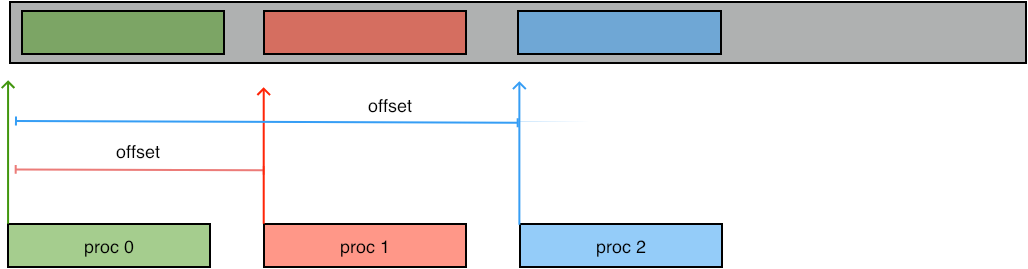
\includegraphics[scale=.4]{write-at-offset}
\end{figure}

\begin{exercise}
  \label{ex:blockwrite}
  Create a buffer of length \n{nwords=3} on each process, and write
  these buffers as a sequence to one file with \indexmpishow{MPI_File_write_at}.
\end{exercise}

Instead of giving the position in the file explicitly, you can also
use a \indexmpishow{MPI_File_seek} call to position the file pointer,
and write with \indexmpishow{MPI_File_write} at the pointer location.
The write call itself also 
\emph{advances the file pointer}\index{file!pointer!advance by write}
so separate calls for writing contiguous elements 
need no seek calls with \indexmpishow{MPI_SEEK_CUR}.

\begin{exercise}
  \label{ex:blockadvance}
  Rewrite the code of exercise~\ref{ex:blockwrite} to
  use a loop where each iteration
  writes only one item to file.
  Note that no explicit advance of the file pointer is needed.
\end{exercise}

\begin{exercise}
  \label{ex:blockseek}
  Construct a file with the consecutive integers $0,\ldots,WP$ where
  $W$~some integer, and $P$~the number of processes. Each process~$p$
  writes the numbers $p,p+W,p+2W,\ldots$. Use a loop where each iteration
  \begin{enumerate}
  \item writes a single number with \lstinline{MPI_File_write}, and
  \item advanced the file pointer with \indexmpishow{MPI_File_seek}
    with a \lstinline{whence} parameter of
    \indexmpishow{MPI_SEEK_CUR}.
  \end{enumerate}
\end{exercise}

\Level 1 {File views}

The previous mode of writing is enough for writing simple contiguous blocks in the file.
However,
you can also access non-contiguous areas in the file. For this you use
%
\indexmpiref{MPI_File_set_view}.
%
This call is collective, even if not all processes access the file.
\begin{itemize}
\item The \n{disp} displacement parameters is measured in bytes. It
  can differ between processes. On sequential files such as tapes or
  network streams it does not make sense to set a displacement; for
  those the \indexmpidef{MPI_DISPLACEMENT_CURRENT} value can be
  used.
\item The \n{etype} describes the data type of the file, it needs to
  be the same on all processes.
\item The \n{filetype} describes how this process sees the file, so it
  can differ between processes.
\item The \n{datarep} string can have the following values:
  \begin{itemize}
  \item \n{native}: data on disk is represented in exactly the same
    format as in memory;
  \item \n{internal}: data on disk is represented in whatever internal
    format is used by the MPI implementation;
  \item \n{external}: data on disk is represented using XDR portable
    data formats.
  \end{itemize}
\item The \n{info} parameter is an \indexmpishow{MPI_Info} object,
  \indexmpishow{MPI_INFO_NULL}.
\end{itemize}

\begin{figure}[ht]
  \label{fig:write-view}
  \caption{Writing at a view}
  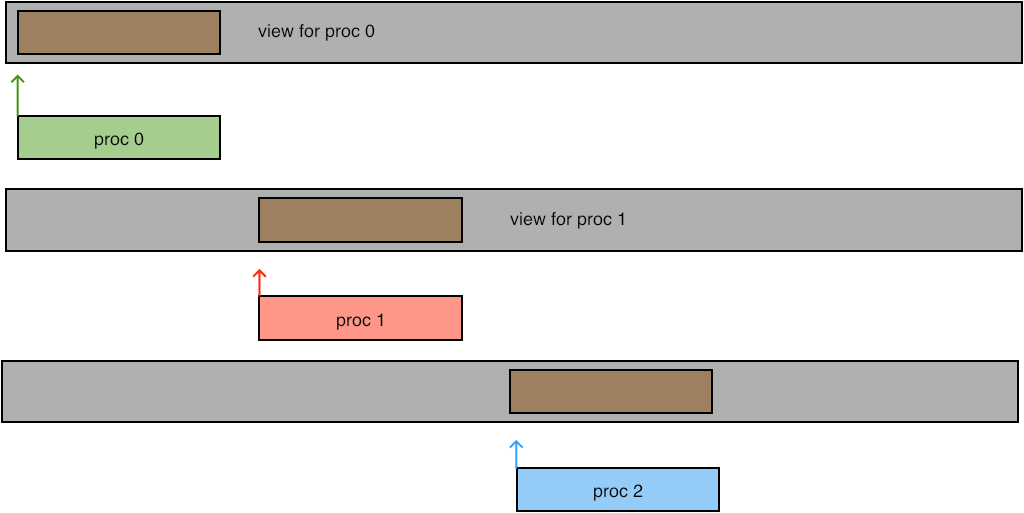
\includegraphics[scale=.4]{write-at-view}
\end{figure}

\begin{exercise}
  \label{ex:viewwrite}
  Write a file in the same way as in exercise~\ref{ex:blockwrite},
  but now use \indexmpishow{MPI_File_write} and use \indexmpishow{MPI_File_set_view} to set
  a view that determines where the data is written.
\end{exercise}

You can get very creative effects by setting the view to a derived
datatype.

\begin{figure}[ht]
  \label{fig:write-derived}
  \caption{Writing at a derived type}
  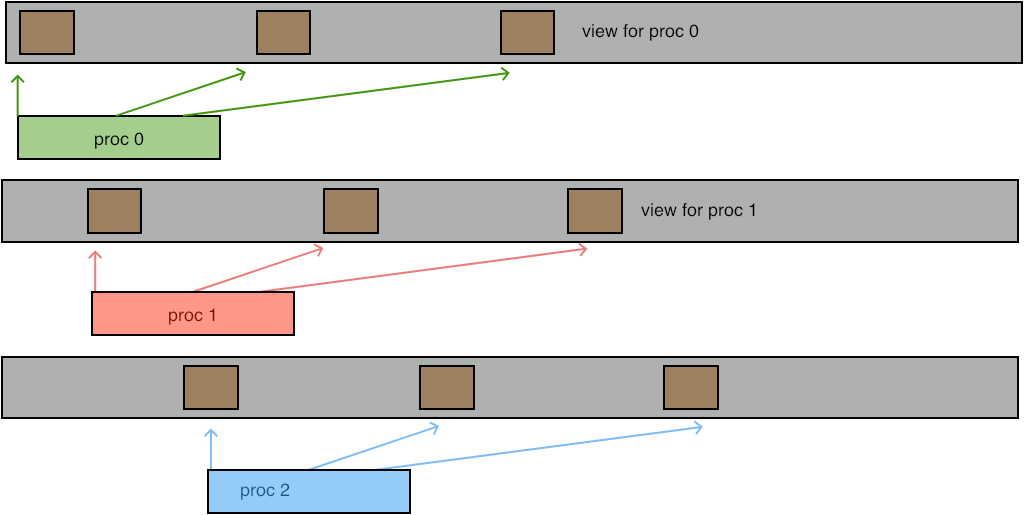
\includegraphics[scale=.4]{write-at-derived}
\end{figure}

\begin{fortrannote}
  In Fortran you have to assure that the displacement parameter is of
  `kind' \indexmpi{MPI_OFFSET_KIND}. In particular, you can not
  specify a literal zero~`0' as the displacement; use
  \indexmpidef{0_MPI_OFFSET_KIND} instead.
\end{fortrannote}

More:
\indexmpishow{MPI_File_set_size}
\indexmpishow{MPI_File_get_size}
\indexmpishow{MPI_File_preallocate}
\indexmpishow{MPI_File_get_view}

\Level 0 {Consistency}

It is possible for one process to read data previously writte by another process.
For this it is of course necessary to impose a temporal order,
for instance by using \indexmpishow{MPI_Barrier},
or using a zero-byte send from the writing to the reading process.

However, the file also needs to be declared atomic:
\indexmpishow{MPI_File_set_atomicity}.

\Level 0 {Constants}

\indexmpishow{MPI_SEEK_SET} used to be called \indextermtt{SEEK_SET}
which gave conflicts with the C++ library. This had to be circumvented
with
\begin{verbatim}
make CPPFLAGS="-DMPICH_IGNORE_CXX_SEEK -DMPICH_SKIP_MPICXX"
\end{verbatim}
and such.

\index{MPI/O|)}
